\section{Benchmark NIST-6 "Boundary Layer"}
\label{sec:bench-6}

This example is a singularly perturbed problem with known exact solution that exhibits
a boundary layer along the right and top sides of the domain.
It is a convection-diffusion equation with first order terms.

\begin{equation} \label{boundary-layer}
-\epsilon \nabla^{2} u + 2\frac{\partial u}{\partial x} + \frac{\partial u}{\partial y} = f 
\end{equation}

in the domain $\Omega = (-1, 1)^2$, equipped with Dirichlet boundary condition
given by the exact solution. The exact solution:

\begin{equation}\label{exact-nist-6}
u(x,y) = (1 - e^{-(1 - x) / \epsilon})(1 - e^{-(1 - y) / \epsilon})cos(\pi (x + y)) 
\end{equation}

where $\epsilon$ determines the strength of the boundary layer.
The right-hand side $f$ is calculated by inserting (\ref{exact-nist-6}) into (\ref{boundary-layer}).
The solution of NIST-6 containing a boundary layer
with $\epsilon = 10^{-1}$ is shown in Fig. \ref{fig:sln-nist06}.

\begin{figure}[!ht]
\centering
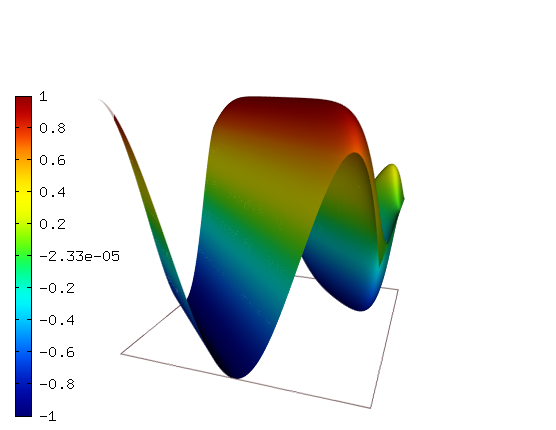
\includegraphics[height=5cm]{nist/nist-6/solution.png}
\caption{The solution to NIST-6 benchmark problem.}
\label{fig:sln-nist06}
\end{figure}

\begin{figure}[!ht]
\centering
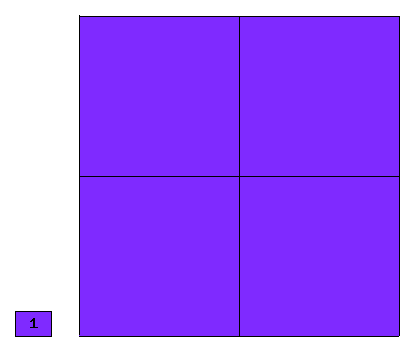
\includegraphics[height=5cm]{nist/nist-6/mesh_hp_aniso_init.png}\ \
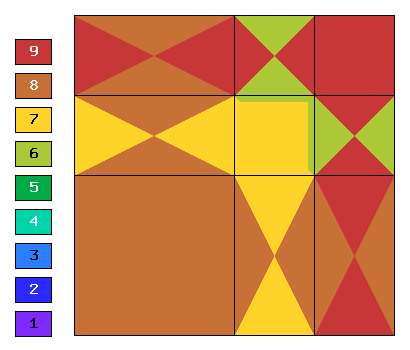
\includegraphics[height=5cm]{nist/nist-6/mesh_hp_aniso.png}
\caption{Initial mesh (left) and final mesh (right) with 591 DOF and the resulting relative error estimate in $H^1$-norm of 6.23458e-04 \% for $hp$-FEM with anisotropic refinements.}
\label{fig:nist-6-hp-aniso}
\end{figure}

\begin{figure}[!ht]
\centering
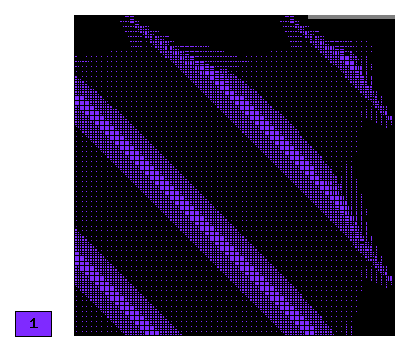
\includegraphics[height=5cm]{nist/nist-6/mesh_h1_aniso.png}\ \
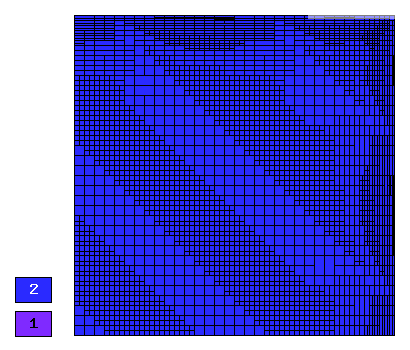
\includegraphics[height=5cm]{nist/nist-6/mesh_h2_aniso.png}
\caption{Final mesh for $h$-FEM with linear and quadratic elements.}
\label{fig:nist-6-h-aniso}
\end{figure}

Figs. \ref{fig:nist-6-conv} compare all
three approaches to automatic adaptivity from the point
of view of DOF and CPU convergence.

\begin{figure}[!ht]
\centering
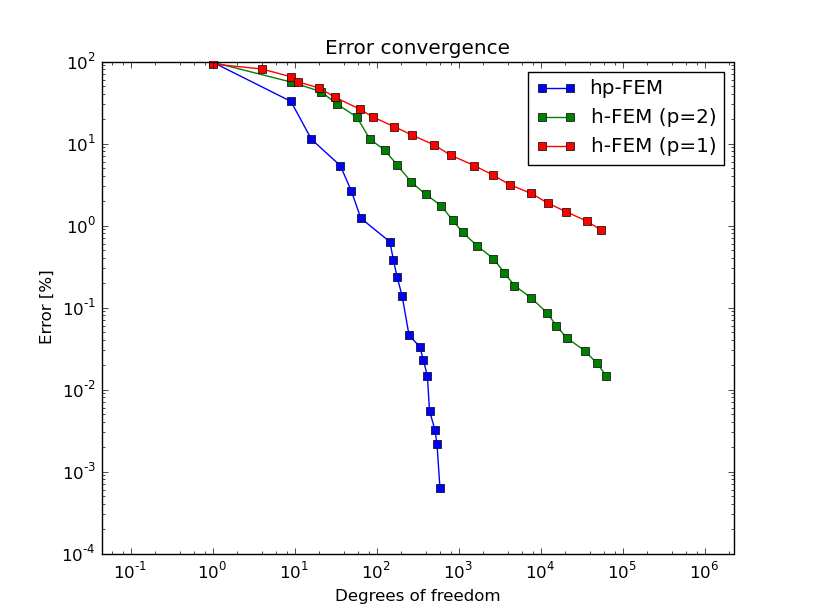
\includegraphics[height=5cm]{nist/nist-6/conv_dof_aniso.png}\ \
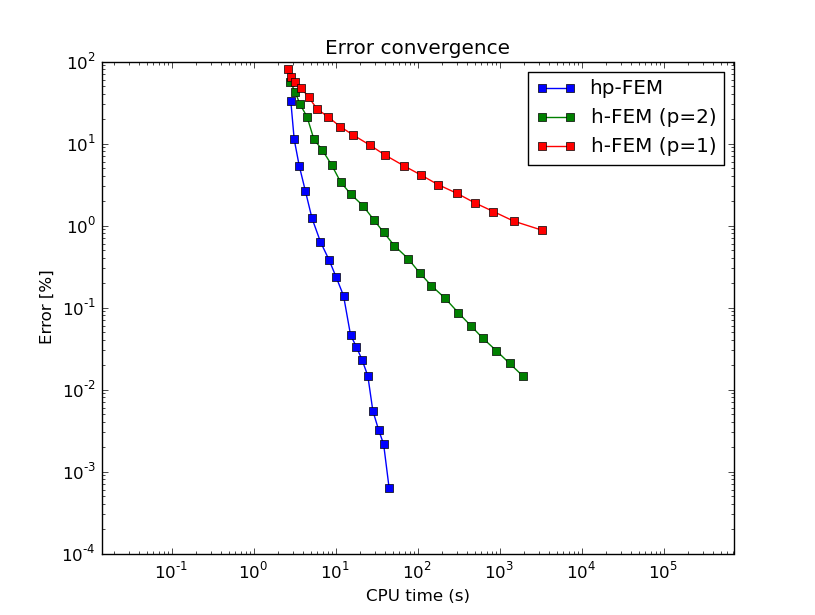
\includegraphics[height=5cm]{nist/nist-6/conv_cpu_aniso.png}
\caption{DOF and CPU time convergence graphs.}
\label{fig:nist-6-conv}
\end{figure}

